\section{连通结构的计算}
\label{sec:graph-connectivity-computation}

第~\ref{sec:graph-connectivity-separation}节把顶点按相互可达划分为连通分量或强连通分量，第~\ref{sec:graph-trees-forests}节说明每个无向分量都有生成树。这些都是存在性的定义。本节把它们算出来：先用遍历给无向图的每个分量编号并抽出生成森林；再处理边不断加入、分量不断合并的情形，引入并查集；最后计算有向图的强连通分量。后一个问题不能简单地重复启动遍历，因为从一个顶点出发能到达的范围，往往大于与它相互可达的范围。

\subsection{连通分量与生成森林}
\label{sec:graph-trav-components-forest}

\paragraph{外层扫描与分量编号}
一次广度或深度优先遍历恰好找出起点所在分量的全部顶点：在无向图中，可达关系是对称的，从$r$可达的顶点就是与$r$相互连通的顶点。要给所有分量编号，只需在外面再套一层扫描。

\begin{algorithm}[无向连通分量编号]
\label{alg:graph-trav-components}
输入：无向图的邻接表。输出：每个顶点的分量编号$\operatorname{comp}(v)$，以及分量数$c$。
\begin{enumerate}
  \item 所有顶点置为未标记，$c=0$。
  \item 按任意固定次序扫描顶点。遇到未标记的顶点$r$时，令$c\gets c+1$，从$r$启动一次广度（或深度）优先遍历，把这次新发现的每个顶点$v$标记为$\operatorname{comp}(v)=c$。已经标记的顶点不再作为起点，也不清除旧编号。
  \item 扫描完全部顶点后输出。
\end{enumerate}
\end{algorithm}

外层扫描必须覆盖全部顶点，否则没有边的孤立点永远不会被任何遍历发现，也就得不到编号。图~\ref{fig:graph-trav-components-forest}中的图由贯穿四点图、一条边$\{5,6\}$和孤立点$7$组成。按编号扫描，从$1$出发的遍历标出$\{1,2,3,4\}$；扫描到$2,3,4$时它们已有编号，跳过；从$5$出发标出$\{5,6\}$；最后$7$自成一个分量。若改变扫描次序，例如先扫描$7$，编号的数值会变，但哪些顶点被分到一起不会变，因为分量本身由图决定。各次遍历合起来把每个顶点和每条邻接记录处理常数次，总时间为$O(n+m)$。

\paragraph{保留发现父边得到生成森林}
遍历时每个新顶点都是经某条边第一次被发现的。把这些父边$\{p(v),v\}$全部保留下来，重复遇到已发现顶点的边一律不加，就得到原图的一个生成森林。

\begin{theorem}[发现父边构成生成森林]
\label{thm:graph-trav-parent-forest}
设对无向图$\mathcal G$执行算法~\ref{alg:graph-trav-components}，并保留所有父边。则这些父边与全部顶点组成$\mathcal G$的一个生成森林，它在每个分量上是一棵生成树，边数为$n-c$。
\end{theorem}

\begin{proof}
每个非起点顶点恰有一条父边，父边的另一端是更早发现的顶点；起点没有父边。于是父边共$n-c$条。

再说明父边不成环。假设某些父边构成一个环，取环上最晚发现的顶点$v$。$v$在环上有两条边，另两端都比$v$早发现。但与$v$相连的父边中，只有$v$自己的父边通向更早发现的顶点，其余父边都是$v$的子顶点的父边，另一端比$v$晚发现。矛盾。

最后，每次遍历从起点出发，沿父指针可以从任何新发现的顶点回到起点，所以每个分量内的父边是连通的。连通、无环、覆盖分量的全部顶点，就是该分量的生成树。
\end{proof}

\begin{figure}[!htb]
  \centering
  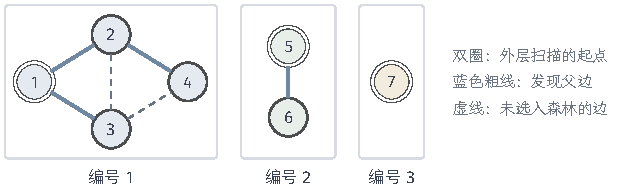
\includegraphics[width=104.8mm]{figures/01-basic-mathematics/04-graphs/tikz/c2-components-spanning-forest/figure.pdf}
  \caption{外层扫描与生成森林。图由贯穿四点图、边$\{5,6\}$和孤立点$7$组成，按编号扫描、每次启动广度优先遍历。三个分量分别获得编号$1,2,3$；双圈是每次遍历的起点，蓝色粗线是保留的父边，共$4=7-3$条，虚线边被检查过但未选入森林。}
  \label{fig:graph-trav-components-forest}
\end{figure}

\paragraph{生成森林丢掉了什么}
图~\ref{fig:graph-trav-components-forest}中第一个分量保留了$\{1,2\}$、$\{1,3\}$、$\{2,4\}$，舍弃了$\{2,3\}$和$\{3,4\}$。生成森林保留了“谁和谁连通”，却不保留其他结构。原图中$3$与$4$直接相邻，在森林中却要走$3\to1\to2\to4$三步；原图没有割点，删去任何一个顶点后其余顶点仍然连通，而在森林中删去$1$或$2$都会把树断开。此外，算法只关心是否连通，边上若有权重，选出的边也没有任何总权最小的保证；在所有生成树中选总权最小的一棵，是第~\ref{sec:graph-minimum-spanning-tree}节的问题。

\subsection{增量连通性与并查集}
\label{sec:graph-trav-union-find}

\paragraph{边不断加入时的分量}
设顶点集固定，边一条一条地加入，每加入一条边后都要回答“两个给定顶点现在是否连通”。每次都重新遍历全图需要$O(n+m)$时间，太浪费。注意加入边$\{u,v\}$对分量的影响很简单：若$u,v$原来已在同一分量，分量不变；否则把两个分量合并成一个。分量构成顶点集的一个划分，加边只会合并其中的两块，不会拆分。于是需要一种数据结构，维护若干互不相交的集合，支持两种操作：$\operatorname{find}(v)$返回$v$所在集合的代表元，两顶点连通当且仅当它们的代表元相同；$\operatorname{union}(u,v)$把$u$和$v$所在的两个集合合并。这种数据结构称为\term{并查集}（union-find），也称不相交集合结构。

\paragraph{父指针树}
并查集把每个集合存成一棵有根树：每个元素保存一个父指针，根的父指针指向自己，根就是集合的代表元。$\operatorname{find}(v)$从$v$出发沿父指针一直走到根；$\operatorname{union}(u,v)$先求出两个根，若不同，就把一个根的父指针改为指向另一个根。这里的父指针只表示“属于同一集合”，与原图的边没有关系：合并$\{1,3\}$时，可能是$3$的根被接到$1$的根下，而原图中这两个根之间未必有边。需要输出原图中的连接时，应另外保存实际加入的边。

\paragraph{按大小合并与路径压缩}
若合并时随意选择谁接到谁下面，树可能退化成一条长链，$\operatorname{find}$要走很多步。两条规则可以避免这一点。

\begin{algorithm}[并查集的两种操作]
\label{alg:graph-trav-union-find}
状态：每个元素$v$的父指针$\operatorname{parent}(v)$，每个根$r$所在集合的大小$\operatorname{size}(r)$。初始时每个元素自成一个集合，$\operatorname{parent}(v)=v$，$\operatorname{size}(v)=1$。
\begin{enumerate}
  \item $\operatorname{find}(v)$：沿父指针从$v$走到根$r$；然后把这条路上经过的每个元素的父指针都直接改为$r$（路径压缩）；返回$r$。
  \item $\operatorname{union}(u,v)$：求$r_u=\operatorname{find}(u)$、$r_v=\operatorname{find}(v)$。若$r_u=r_v$，不做任何事。否则把较小集合的根接到较大集合的根下，大小相同时把$r_v$接到$r_u$下（按大小合并），并把新根的大小更新为两者之和。
\end{enumerate}
\end{algorithm}

图~\ref{fig:graph-trav-union-find}按边序列$\{1,2\}$、$\{3,4\}$、$\{1,3\}$、$\{5,6\}$、$\{4,6\}$追踪这些操作。前两次合并各把一个单点接到另一个单点下，得到$\{1,2\}$与$\{3,4\}$，此时还有单点集合$\{5\}$、$\{6\}$。合并$\{1,3\}$时两个集合大小都是$2$，按约定把根$3$接到根$1$下，$4$的深度变为$2$。之后若查询$\operatorname{find}(4)$，沿$4\to3\to1$找到根$1$，路径压缩把$4$的父指针直接改为$1$，下次查询只需一步。合并$\{5,6\}$得到大小为$2$的集合；处理$\{4,6\}$时，$4$所在集合大小为$4$、$6$所在集合大小为$2$，于是根$5$接到根$1$下，全部六个元素属于同一集合。每一步后的集合划分都与“已加入的边构成的图的连通分量”一致。

\begin{figure}[!htb]
  \centering
  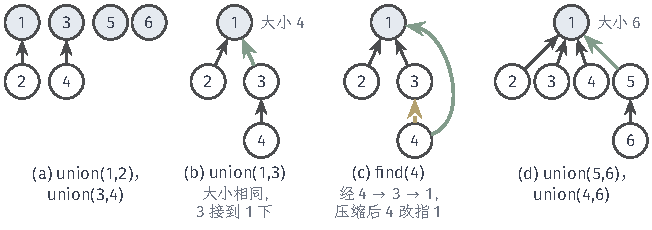
\includegraphics[width=110.5mm]{figures/01-basic-mathematics/04-graphs/tikz/c2-union-find/figure.pdf}
  \caption{并查集的父指针树，箭头由元素指向其父指针，蓝色填充为根。(a)合并$\{1,2\}$、$\{3,4\}$后；(b)合并两个大小为$2$的集合，按约定把根$3$接到根$1$下（绿色箭头）；(c)查询$\operatorname{find}(4)$经过$4\to3\to1$（黄色虚线是原父指针），路径压缩后$4$直接指向根$1$；(d)合并$\{5,6\}$后再处理$\{4,6\}$，较小集合的根$5$接到较大集合的根$1$下。}
  \label{fig:graph-trav-union-find}
\end{figure}

\paragraph{树高与操作开销}
按大小合并能保证树不会太高。

\begin{theorem}[按大小合并的树高]
\label{thm:graph-trav-union-by-size}
只使用按大小合并（无论是否路径压缩）时，任一元素到根的路径长度不超过$\log_2 n$，其中$n$是元素总数。
\end{theorem}

\begin{proof}
先不考虑路径压缩。一个元素的深度只在它所在的根被接到另一个根下面时增加$1$；按规则，被接的那一侧不大于另一侧，所以合并后该元素所在集合的大小至少是原来的两倍。集合大小从$1$开始，不超过$n$，至多翻倍$\log_2 n$次，深度也就至多为$\log_2 n$。路径压缩只把元素的父指针改为它的某个祖先，只会让深度变小，不影响这个上界。
\end{proof}

因此每次$\operatorname{find}$和$\operatorname{union}$都只需$O(\log n)$时间，存储为$O(n)$。路径压缩使反复查询同一区域变得更快。可以证明，两条规则同时使用时，任意$k$次操作的总时间为$O(k\,\alpha(n))$，其中$\alpha$是增长极慢的反Ackermann函数，对任何实际规模的$n$都不超过$4$；这一摊还分析较长，这里不展开，使用时只需记住每次操作的平均代价几乎是常数。

\paragraph{适用范围}
并查集适合“只加边、不删边”的情形。第~\ref{sec:graph-minimum-spanning-tree}节的Kruskal算法按边权从小到大考虑每条边，需要判断加入这条边是否会成环，也就是判断两个端点是否已在同一分量，正好用并查集完成。删除一条边可能把一个分量拆成两个，而并查集的合并无法撤销，所以它不能直接维护任意删边后的分量。在图像中给相连的像素区域编号时，也常先给像素临时标号、再用并查集合并相遇的标号，具体扫描方式留到应用部分。

\subsection{强连通分量与缩点}
\label{sec:graph-trav-scc}

\paragraph{一次搜索为什么不够}
在有向图中，从顶点$v$出发的一次遍历找到的是$v$能到达的全部顶点，而$v$所在的强连通分量要求双向可达。图~\ref{fig:graph-trav-kosaraju}(a)中，从$1$出发的深度优先遍历依次发现$1,2,3,4$，但$3,4$回不到$1$，$1$所在的强连通分量只是$\{1,2\}$。一般地，$v$所在的强分量等于“从$v$可达的顶点”与“能到达$v$的顶点”的交集；后者可以在把所有弧反向后的图上从$v$遍历得到。对每个顶点都这样做两次遍历需要$O(n(n+m))$时间。下面的算法只用两遍深度优先遍历，在$O(n+m)$时间内求出全部强连通分量。

\paragraph{两遍深度优先遍历}
把有向图$\mathcal G$的每条弧$u\to v$改为$v\to u$，得到\term{反向图}（reverse graph）$\mathcal G^{\mathrm{rev}}$。$\mathcal G$与$\mathcal G^{\mathrm{rev}}$的强连通分量相同，因为相互可达的两个顶点在弧全部反向后仍然相互可达。算法的第一遍在原图上计算完成时刻，第二遍在反向图上按完成时刻从大到小选择起点。这一方法称为\term{Kosaraju算法}（Kosaraju's algorithm）。

\begin{algorithm}[Kosaraju强连通分量算法]
\label{alg:graph-trav-kosaraju}
输入：有向图$\mathcal G=(V,E)$的出邻接表。输出：每个顶点所属强连通分量的编号。
\begin{enumerate}
  \item 在$\mathcal G$上执行完整的深度优先遍历（算法~\ref{alg:graph-trav-dfs}），覆盖全部顶点，记录完成次序。
  \item 扫描出邻接表，构造反向图$\mathcal G^{\mathrm{rev}}$的出邻接表，即原图的入邻接表。
  \item 所有顶点置为未标记。按完成时刻从大到小扫描顶点；遇到未标记的顶点$r$时，开始一个新分量，在$\mathcal G^{\mathrm{rev}}$上从$r$遍历（广度或深度优先均可），只进入未标记的顶点，把这次到达的顶点全部标为这个分量。
\end{enumerate}
\end{algorithm}

\paragraph{在三个强分量组成的图上追踪}
图~\ref{fig:graph-trav-kosaraju}的有向图有七个顶点，弧为$1\to2$、$2\to1$、$2\to3$、$3\to4$、$4\to3$、$5\to6$、$6\to4$、$6\to7$、$7\to1$、$7\to5$。它的强连通分量是$\{5,6,7\}$、$\{1,2\}$和$\{3,4\}$，分量之间只有单向的弧。

第一遍按编号选择起点、按编号读取出邻居。从$1$出发，依次发现$1,2,3,4$；$4$的出邻居$3$在栈中，$4$完成，随后$3,2,1$依次完成，完成时刻为$f(4)=5$、$f(3)=6$、$f(2)=7$、$f(1)=8$。接着从$5$重新出发，发现$5,6$；$6$的出邻居$4$已完成，跳过，再发现$7$；$7$的出邻居$1$已完成、$5$在栈中，于是$7,6,5$依次完成，$f(7)=12$、$f(6)=13$、$f(5)=14$。完成次序为$4,3,2,1,7,6,5$，见图~\ref{fig:graph-trav-kosaraju}(a)。

第二遍按完成时刻从大到小，即$5,6,7,1,2,3,4$选择起点，在反向图上遍历，见图~\ref{fig:graph-trav-kosaraju}(b)。从$5$出发，反向弧把它引向$7$，再引向$6$；$\{5,6,7\}$中没有反向弧通往别处，于是得到第一个分量$\{5,6,7\}$。下一个未标记的是$1$：反向弧$1\to2$、$1\to7$中$7$已标记，只进入$2$，得到$\{1,2\}$。最后从$3$出发，反向弧$3\to2$通往已标记的$2$，只进入$4$，得到$\{3,4\}$。每次遍历恰好停在一个强分量的边界上。若第二遍在原图而不是反向图上从$5$遍历，会经$6\to4$、$7\to1$走进另外两个分量，所以反向这一步不可省略。

\begin{figure*}[!htb]
  \centering
  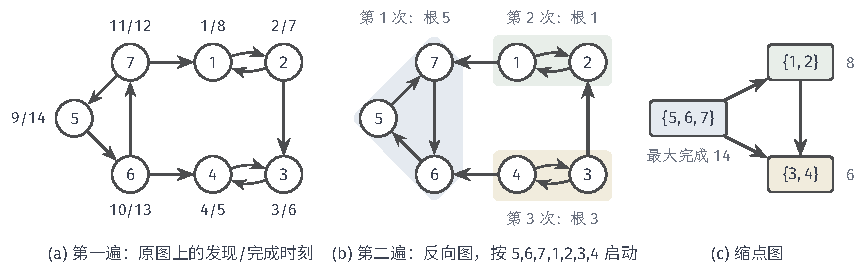
\includegraphics[width=146.5mm]{figures/01-basic-mathematics/04-graphs/tikz/c2-kosaraju-condensation/figure.pdf}
  \caption{Kosaraju算法的两遍过程与缩点图。(a)原图上按编号重启的深度优先遍历，顶点旁为发现/完成时刻；粗箭头是连接不同强分量的弧。(b)反向图上按完成时刻从大到小（$5,6,7,1,2,3,4$）选择起点，三次遍历分别得到蓝、绿、黄三个强连通分量，指向已标记分量的反向弧不再进入。(c)把每个强分量缩成一点得到的缩点图，旁注为各分量中最大的完成时刻；缩点图无环，且最大完成时刻沿弧方向递减。}
  \label{fig:graph-trav-kosaraju}
\end{figure*}

\paragraph{完成次序的性质}
第二遍之所以不会越界，是因为第一遍的完成时刻在分量之间有固定的先后。对强连通分量$C$，记$f(C)=\max_{v\in C}f(v)$为其中最大的完成时刻。在上例中，$f(\{5,6,7\})=14$、$f(\{1,2\})=8$、$f(\{3,4\})=6$，而分量之间的弧都从$f$值大的指向$f$值小的。

\begin{lemma}[分量间的完成时刻]
\label{lem:graph-trav-scc-finish}
设$C\neq C'$是有向图的两个强连通分量，且存在一条从$C$中顶点指向$C'$中顶点的弧。则在一次完整的深度优先遍历中，$f(C)>f(C')$。
\end{lemma}

\begin{proof}
考察$C\cup C'$中最先被发现的顶点$x$。

若$x\in C$。在时刻$d(x)$，$C\cup C'$中其余顶点都未发现。$C$中每个顶点都能从$x$经$C$内部的路径到达；$C'$中每个顶点都能先在$C$内走到那条弧的起点，经弧进入$C'$，再在$C'$内部到达。这些路径上的顶点此时都未发现，由引理~\ref{lem:graph-trav-white-path}，$C\cup C'$中其余顶点都成为$x$的后代并先于$x$完成，所以$f(C)=f(x)>f(C')$。

若$x\in C'$。同理，$C'$中其余顶点都成为$x$的后代，$f(C')=f(x)$。另一方面，从$C'$中的任何顶点都不能到达$C$：否则结合已有的从$C$到$C'$的弧，$C$与$C'$中的顶点相互可达，它们就应属于同一个强分量。所以在$x$处于处理中期间，$C$中没有顶点被发现（那样的顶点会是$x$的后代，从而从$x$可达）。$C$中顶点都在$f(x)$之后才被发现，也就在$f(x)$之后完成，所以$f(C)>f(x)=f(C')$。
\end{proof}

\paragraph{第二遍为什么恰好取出一个分量}
在反向图中，引理~\ref{lem:graph-trav-scc-finish}的不等式方向随弧一起反转：从分量$C$出发的反向弧只能通往$f$值更大的分量。第二遍按$f$值从大到小选择起点，这些分量在轮到$C$之前都已标记，于是遍历被挡在$C$之内。

\begin{theorem}[Kosaraju算法的正确性]
\label{thm:graph-trav-kosaraju}
算法~\ref{alg:graph-trav-kosaraju}第三步的每一次遍历，恰好标记一个强连通分量的全部顶点。
\end{theorem}

\begin{proof}
对第二遍已经完成的遍历次数归纳，假设此前每次遍历都恰好标记了一个完整的强分量。设下一个起点是$r$，所在分量为$C$。$r$是未标记顶点中完成时刻最大的；由归纳假设，未标记的顶点恰好组成若干个完整的强分量，所以$f(r)=f(C)$，且$C$在未标记的分量中$f$值最大。

$C$在反向图中仍然强连通，从$r$出发能到达$C$的全部顶点，而$C$中的顶点都未标记，因此都会被这次遍历标记。另一方面，设反向图中有一条弧从$C$中顶点指向另一个分量$C'$中的顶点，它对应原图中一条从$C'$指向$C$的弧，由引理~\ref{lem:graph-trav-scc-finish}有$f(C')>f(C)$。而$C$是未标记分量中$f$值最大的，所以$C'$已经被标记，这次遍历不会进入。因此这次遍历标记的恰好是$C$。
\end{proof}

\paragraph{计算开销}
第一遍深度优先遍历用$O(n+m)$时间。构造反向图需要扫描每条弧一次，时间与额外存储都是$O(n+m)$。第二遍按完成时刻从大到小扫描，只需把第一遍的完成次序倒过来读，不必排序；遍历本身再用$O(n+m)$时间。总时间为$O(n+m)$。三处细节缺一不可：第一遍必须覆盖全部顶点，否则有些顶点没有完成时刻；第二遍必须在反向图上进行；起点必须按完成时刻从大到小选择，若改为从小到大，上例中第二遍会先从$4$出发，在反向图上经$4\to6$进入$\{5,6,7\}$，再经$3\to2$进入$\{1,2\}$，把三个分量全部混在一起。

\paragraph{缩点图}
得到强连通分量后，可以把每个分量看成一个整体。把每个强分量压缩为一个顶点，若原图中有从分量$C$指向另一分量$C'$的弧，就在$C$与$C'$之间连一条弧$C\to C'$（多条这样的弧只保留一条，分量内部的弧舍去），得到的有向图称为\term{缩点图}（condensation graph）。图~\ref{fig:graph-trav-kosaraju}(c)中，缩点图有三个顶点和三条弧$\{5,6,7\}\to\{1,2\}$、$\{1,2\}\to\{3,4\}$、$\{5,6,7\}\to\{3,4\}$。

\begin{theorem}[缩点图无环]
\label{thm:graph-trav-condensation-dag}
任何有限有向图的缩点图都是有向无环图。
\end{theorem}

\begin{proof}
假设缩点图中有有向环$C_1\to C_2\to\cdots\to C_k\to C_1$，$k\geq2$，各$C_i$是不同的强分量。每条弧$C_i\to C_{i+1}$对应原图中一条从$C_i$中某顶点到$C_{i+1}$中某顶点的弧，而每个分量内部任意两点相互可达。于是从$C_1$中任一顶点出发，可以依次经过$C_2,\ldots,C_k$再回到$C_1$，环上所有分量中的顶点两两相互可达，它们应属于同一个强分量，与$C_1,\ldots,C_k$互不相同矛盾。
\end{proof}

由引理~\ref{lem:graph-trav-scc-finish}，缩点图中每条弧都从$f$值较大的分量指向$f$值较小的分量，所以Kosaraju算法第二遍得到分量的先后次序，恰好使缩点图的每条弧从先得到的分量指向后得到的分量。上例中得到的次序$\{5,6,7\}$、$\{1,2\}$、$\{3,4\}$就满足这一点。任何有向图都可以先缩点、再在无环的缩点图上安排先后，这正是下一节要研究的依赖排序。
